% Options for packages loaded elsewhere
\PassOptionsToPackage{unicode}{hyperref}
\PassOptionsToPackage{hyphens}{url}
\PassOptionsToPackage{dvipsnames,svgnames,x11names}{xcolor}
%
\documentclass[
  letterpaper,
  DIV=11,
  numbers=noendperiod]{scrartcl}

\usepackage{amsmath,amssymb}
\usepackage{lmodern}
\usepackage{iftex}
\ifPDFTeX
  \usepackage[T1]{fontenc}
  \usepackage[utf8]{inputenc}
  \usepackage{textcomp} % provide euro and other symbols
\else % if luatex or xetex
  \usepackage{unicode-math}
  \defaultfontfeatures{Scale=MatchLowercase}
  \defaultfontfeatures[\rmfamily]{Ligatures=TeX,Scale=1}
\fi
% Use upquote if available, for straight quotes in verbatim environments
\IfFileExists{upquote.sty}{\usepackage{upquote}}{}
\IfFileExists{microtype.sty}{% use microtype if available
  \usepackage[]{microtype}
  \UseMicrotypeSet[protrusion]{basicmath} % disable protrusion for tt fonts
}{}
\makeatletter
\@ifundefined{KOMAClassName}{% if non-KOMA class
  \IfFileExists{parskip.sty}{%
    \usepackage{parskip}
  }{% else
    \setlength{\parindent}{0pt}
    \setlength{\parskip}{6pt plus 2pt minus 1pt}}
}{% if KOMA class
  \KOMAoptions{parskip=half}}
\makeatother
\usepackage{xcolor}
\setlength{\emergencystretch}{3em} % prevent overfull lines
\setcounter{secnumdepth}{-\maxdimen} % remove section numbering
% Make \paragraph and \subparagraph free-standing
\ifx\paragraph\undefined\else
  \let\oldparagraph\paragraph
  \renewcommand{\paragraph}[1]{\oldparagraph{#1}\mbox{}}
\fi
\ifx\subparagraph\undefined\else
  \let\oldsubparagraph\subparagraph
  \renewcommand{\subparagraph}[1]{\oldsubparagraph{#1}\mbox{}}
\fi

\usepackage{color}
\usepackage{fancyvrb}
\newcommand{\VerbBar}{|}
\newcommand{\VERB}{\Verb[commandchars=\\\{\}]}
\DefineVerbatimEnvironment{Highlighting}{Verbatim}{commandchars=\\\{\}}
% Add ',fontsize=\small' for more characters per line
\usepackage{framed}
\definecolor{shadecolor}{RGB}{241,243,245}
\newenvironment{Shaded}{\begin{snugshade}}{\end{snugshade}}
\newcommand{\AlertTok}[1]{\textcolor[rgb]{0.68,0.00,0.00}{#1}}
\newcommand{\AnnotationTok}[1]{\textcolor[rgb]{0.37,0.37,0.37}{#1}}
\newcommand{\AttributeTok}[1]{\textcolor[rgb]{0.40,0.45,0.13}{#1}}
\newcommand{\BaseNTok}[1]{\textcolor[rgb]{0.68,0.00,0.00}{#1}}
\newcommand{\BuiltInTok}[1]{\textcolor[rgb]{0.00,0.23,0.31}{#1}}
\newcommand{\CharTok}[1]{\textcolor[rgb]{0.13,0.47,0.30}{#1}}
\newcommand{\CommentTok}[1]{\textcolor[rgb]{0.37,0.37,0.37}{#1}}
\newcommand{\CommentVarTok}[1]{\textcolor[rgb]{0.37,0.37,0.37}{\textit{#1}}}
\newcommand{\ConstantTok}[1]{\textcolor[rgb]{0.56,0.35,0.01}{#1}}
\newcommand{\ControlFlowTok}[1]{\textcolor[rgb]{0.00,0.23,0.31}{#1}}
\newcommand{\DataTypeTok}[1]{\textcolor[rgb]{0.68,0.00,0.00}{#1}}
\newcommand{\DecValTok}[1]{\textcolor[rgb]{0.68,0.00,0.00}{#1}}
\newcommand{\DocumentationTok}[1]{\textcolor[rgb]{0.37,0.37,0.37}{\textit{#1}}}
\newcommand{\ErrorTok}[1]{\textcolor[rgb]{0.68,0.00,0.00}{#1}}
\newcommand{\ExtensionTok}[1]{\textcolor[rgb]{0.00,0.23,0.31}{#1}}
\newcommand{\FloatTok}[1]{\textcolor[rgb]{0.68,0.00,0.00}{#1}}
\newcommand{\FunctionTok}[1]{\textcolor[rgb]{0.28,0.35,0.67}{#1}}
\newcommand{\ImportTok}[1]{\textcolor[rgb]{0.00,0.46,0.62}{#1}}
\newcommand{\InformationTok}[1]{\textcolor[rgb]{0.37,0.37,0.37}{#1}}
\newcommand{\KeywordTok}[1]{\textcolor[rgb]{0.00,0.23,0.31}{#1}}
\newcommand{\NormalTok}[1]{\textcolor[rgb]{0.00,0.23,0.31}{#1}}
\newcommand{\OperatorTok}[1]{\textcolor[rgb]{0.37,0.37,0.37}{#1}}
\newcommand{\OtherTok}[1]{\textcolor[rgb]{0.00,0.23,0.31}{#1}}
\newcommand{\PreprocessorTok}[1]{\textcolor[rgb]{0.68,0.00,0.00}{#1}}
\newcommand{\RegionMarkerTok}[1]{\textcolor[rgb]{0.00,0.23,0.31}{#1}}
\newcommand{\SpecialCharTok}[1]{\textcolor[rgb]{0.37,0.37,0.37}{#1}}
\newcommand{\SpecialStringTok}[1]{\textcolor[rgb]{0.13,0.47,0.30}{#1}}
\newcommand{\StringTok}[1]{\textcolor[rgb]{0.13,0.47,0.30}{#1}}
\newcommand{\VariableTok}[1]{\textcolor[rgb]{0.07,0.07,0.07}{#1}}
\newcommand{\VerbatimStringTok}[1]{\textcolor[rgb]{0.13,0.47,0.30}{#1}}
\newcommand{\WarningTok}[1]{\textcolor[rgb]{0.37,0.37,0.37}{\textit{#1}}}

\providecommand{\tightlist}{%
  \setlength{\itemsep}{0pt}\setlength{\parskip}{0pt}}\usepackage{longtable,booktabs,array}
\usepackage{calc} % for calculating minipage widths
% Correct order of tables after \paragraph or \subparagraph
\usepackage{etoolbox}
\makeatletter
\patchcmd\longtable{\par}{\if@noskipsec\mbox{}\fi\par}{}{}
\makeatother
% Allow footnotes in longtable head/foot
\IfFileExists{footnotehyper.sty}{\usepackage{footnotehyper}}{\usepackage{footnote}}
\makesavenoteenv{longtable}
\usepackage{graphicx}
\makeatletter
\def\maxwidth{\ifdim\Gin@nat@width>\linewidth\linewidth\else\Gin@nat@width\fi}
\def\maxheight{\ifdim\Gin@nat@height>\textheight\textheight\else\Gin@nat@height\fi}
\makeatother
% Scale images if necessary, so that they will not overflow the page
% margins by default, and it is still possible to overwrite the defaults
% using explicit options in \includegraphics[width, height, ...]{}
\setkeys{Gin}{width=\maxwidth,height=\maxheight,keepaspectratio}
% Set default figure placement to htbp
\makeatletter
\def\fps@figure{htbp}
\makeatother
\newlength{\cslhangindent}
\setlength{\cslhangindent}{1.5em}
\newlength{\csllabelwidth}
\setlength{\csllabelwidth}{3em}
\newlength{\cslentryspacingunit} % times entry-spacing
\setlength{\cslentryspacingunit}{\parskip}
\newenvironment{CSLReferences}[2] % #1 hanging-ident, #2 entry spacing
 {% don't indent paragraphs
  \setlength{\parindent}{0pt}
  % turn on hanging indent if param 1 is 1
  \ifodd #1
  \let\oldpar\par
  \def\par{\hangindent=\cslhangindent\oldpar}
  \fi
  % set entry spacing
  \setlength{\parskip}{#2\cslentryspacingunit}
 }%
 {}
\usepackage{calc}
\newcommand{\CSLBlock}[1]{#1\hfill\break}
\newcommand{\CSLLeftMargin}[1]{\parbox[t]{\csllabelwidth}{#1}}
\newcommand{\CSLRightInline}[1]{\parbox[t]{\linewidth - \csllabelwidth}{#1}\break}
\newcommand{\CSLIndent}[1]{\hspace{\cslhangindent}#1}

\usepackage{hyperref}
\usepackage{caption}
\usepackage{subcaption}
\usepackage{algorithm}
\usepackage{algpseudocode}
\KOMAoption{captions}{tableheading}
\makeatletter
\makeatother
\makeatletter
\makeatother
\makeatletter
\@ifpackageloaded{caption}{}{\usepackage{caption}}
\AtBeginDocument{%
\ifdefined\contentsname
  \renewcommand*\contentsname{Table of contents}
\else
  \newcommand\contentsname{Table of contents}
\fi
\ifdefined\listfigurename
  \renewcommand*\listfigurename{List of Figures}
\else
  \newcommand\listfigurename{List of Figures}
\fi
\ifdefined\listtablename
  \renewcommand*\listtablename{List of Tables}
\else
  \newcommand\listtablename{List of Tables}
\fi
\ifdefined\figurename
  \renewcommand*\figurename{Figure}
\else
  \newcommand\figurename{Figure}
\fi
\ifdefined\tablename
  \renewcommand*\tablename{Table}
\else
  \newcommand\tablename{Table}
\fi
}
\@ifpackageloaded{float}{}{\usepackage{float}}
\floatstyle{ruled}
\@ifundefined{c@chapter}{\newfloat{codelisting}{h}{lop}}{\newfloat{codelisting}{h}{lop}[chapter]}
\floatname{codelisting}{Listing}
\newcommand*\listoflistings{\listof{codelisting}{List of Listings}}
\usepackage{amsthm}
\theoremstyle{plain}
\newtheorem{corollary}{Corollary}[section]
\theoremstyle{plain}
\newtheorem{proposition}{Proposition}[section]
\theoremstyle{plain}
\newtheorem{lemma}{Lemma}[section]
\theoremstyle{definition}
\newtheorem{definition}{Definition}[section]
\theoremstyle{plain}
\newtheorem{theorem}{Theorem}[section]
\theoremstyle{remark}
\renewcommand*{\proofname}{Proof}
\newtheorem*{remark}{Remark}
\newtheorem*{solution}{Solution}
\makeatother
\makeatletter
\@ifpackageloaded{caption}{}{\usepackage{caption}}
\@ifpackageloaded{subcaption}{}{\usepackage{subcaption}}
\makeatother
\makeatletter
\@ifpackageloaded{tcolorbox}{}{\usepackage[many]{tcolorbox}}
\makeatother
\makeatletter
\@ifundefined{shadecolor}{\definecolor{shadecolor}{rgb}{.97, .97, .97}}
\makeatother
\makeatletter
\makeatother
\ifLuaTeX
  \usepackage{selnolig}  % disable illegal ligatures
\fi
\IfFileExists{bookmark.sty}{\usepackage{bookmark}}{\usepackage{hyperref}}
\IfFileExists{xurl.sty}{\usepackage{xurl}}{} % add URL line breaks if available
\urlstyle{same} % disable monospaced font for URLs
\hypersetup{
  pdftitle={Twice Ramanujan Sparsifiers},
  pdfauthor={Hamid R. Kamkari, Amandeep Singh},
  colorlinks=true,
  linkcolor={blue},
  filecolor={Maroon},
  citecolor={Blue},
  urlcolor={Blue},
  pdfcreator={LaTeX via pandoc}}

\title{Twice Ramanujan Sparsifiers\thanks{We have published this
document as a blog post in our repository using Quarto, for a better
visualization and implementations please check out our post at
\url{https://hamidrezakmk.github.io/twice-ramanujan-sparsifiers/docs/}}}
\author{Hamid R. Kamkari, Amandeep Singh}
\date{}

\begin{document}
\maketitle
\ifdefined\Shaded\renewenvironment{Shaded}{\begin{tcolorbox}[borderline west={3pt}{0pt}{shadecolor}, enhanced, boxrule=0pt, sharp corners, breakable, frame hidden, interior hidden]}{\end{tcolorbox}}\fi

For any graph \(G\) a sparsifier \(H\) is a graph with far fewer edges
that is similar to \(G\) in some useful way. While \(H\) is much easier
to do computation on, it holds the same properties as \(G\), and
therefore, it is a reliable way of doing approximate computation on
\(G\). For example, if we are dealing with path-finding problems on a
dense large graph \(G\), the set of sparsifiers used in (Chew 1989) can
be used because they are guaranteed to have almost the same shortest
path properties as \(G\).

For illustration, consider the following graph \(G\) with four vertices.
The new graph obtained has far fewer edges but has the same set of
shortest paths between any pair of vertices. This is a simple sparsifier
that can be used for shortest path-finding problems and can be obtained
via removing trivial edges \(w(u,v)\) such that the shortest distance
between \(u\) and \(v\) is smaller than or equal to \(w(u,v)\).


\begin{figure}

\begin{minipage}[t]{0.50\linewidth}

{\centering 

\raisebox{-\height}{

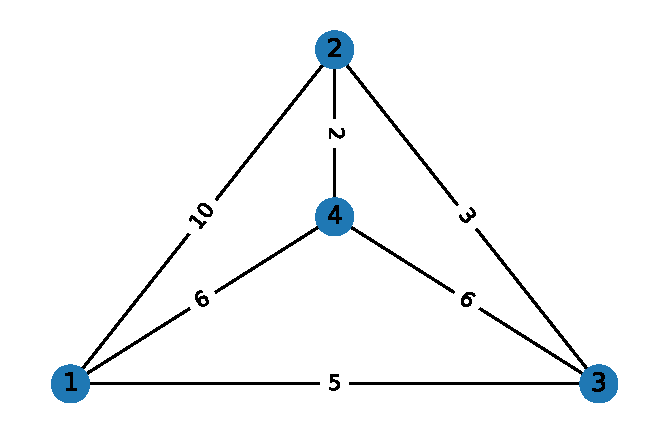
\includegraphics{index_files/figure-pdf/fig-shortest-path-sparsification-output-1.pdf}

}

}

\subcaption{\label{fig-shortest-path-sparsification-1}The graph \(G\)
that we intend to sparsify.}
\end{minipage}%
%
\begin{minipage}[t]{0.50\linewidth}

{\centering 

\raisebox{-\height}{

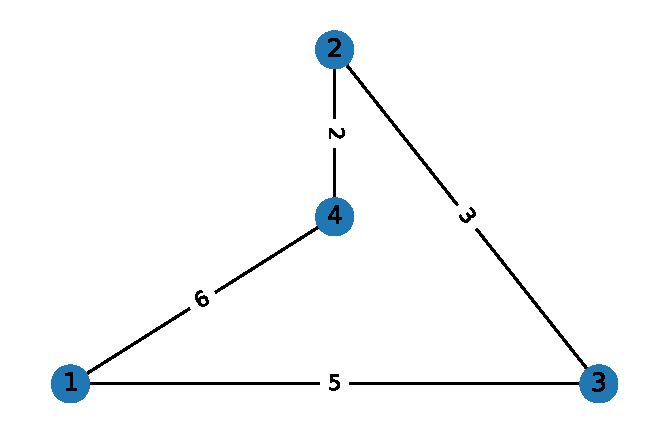
\includegraphics{index_files/figure-pdf/fig-shortest-path-sparsification-output-2.pdf}

}

}

\subcaption{\label{fig-shortest-path-sparsification-2}The graph \(H\)
that is obtained by removing trivial edges.}
\end{minipage}%

\caption{\label{fig-shortest-path-sparsification}A simple illustration
of a sparsifier that can help with shortest path problems.}

\end{figure}

On the other hand, (Benczúr and Karger 1996) for example introduces the
cut-sparsifiers which are a class of sparsifiers that have almost
identical cut weights for any set \(S \subset V\) meaning that
\(E_G(S, \bar{S}) \approx E_H(S, \bar{S})\). In this write-up, we cover
spectral graph sparsifiers which are a certain class of sparsifiers that
have a tight connection with expander graphs and can approximate the
Laplacian of a graph with high accuracy. These sparsifiers preserve
random walk properties as well and can be used as a substitute for
original graphs in many applications such as recently in Graph Neural
Networks (GNNs) (Li et al. 2020).

Because of the close connection between graph spectral connectivity and
edge connectivity introduced by Cheeger (Cheeger 1970), spectral
sparsifiers were introduced by (Spielman and Teng 2004) and (Spielman
and Teng 2011) as an important tool. Conventionally, these graphs are
constructed using randomized algorithms where we pick a certain edge of
an original graph with a probability and sample edges until we obtain a
good approximation. For example, if an edge is crucial to the
connectivity of our graph, then it has high importance and should be
picked with high probability. However, in this write-up, we will show
that we can construct a sparsifier with a deterministic algorithm
introduced in (Batson, Spielman, and Srivastava 2009) that has a tight
connection with the Ramanujan bounds.

Furthermore, we will cover an important reduction from the graph
sparsification problem to a matrix approximation problem which has been
further exploder in many follow-up papers (Tat Lee and Sun 2015) and
(Lee and Sun 2017). Moreover, this will give us the first deterministic
algorithm for obtaining sparsifiers with a linear number of edges. That
said, we have implemented the algorithm in Python and have tested it on
a few graphs for illustration purposes and our package is available in
our
\href{https://github.com/HamidrezaKmK/twice-ramanujan-sparsifiers}{Github
repository}.

Finally, we will focus our attention on running the algorithm on
complete graphs. The sparsifier obtained from the complete graph will
have high connectivity which resembles similarities with the expander
graphs. Although the graph obtained from the algorithm is not regular,
we will show that it has a lot of expander-like properties and we will
draw a close connection with Ramanujan graphs.

\hypertarget{recap-and-preliminaries}{%
\subsection{Recap and Preliminaries}\label{recap-and-preliminaries}}

Here we will cover some preliminaries on spectral sparsification and
then we will discuss the effective resistance-based algorithm for
spectral sparsification. We will also discuss an important reduction to
the matrix problem which lays the groundwork for the final algorithm.

\hypertarget{spectral-sparsification}{%
\subsubsection{Spectral Sparsification}\label{spectral-sparsification}}

Before everything, we should define what a spectral sparsifier is. A
spectral sparsifier is a sparse graph that approximates the Laplacian of
a graph with high accuracy. In other words, a sparsifier is a graph that
has a lot of the same properties as the original graph; formally,

\leavevmode\vadjust pre{\hypertarget{def-spectral-sparsification}{}}%
\begin{definition}[]\label{def-spectral-sparsification}

A \((k, \epsilon)\)-spectral sparsifier of a graph \(G = (V, E, w)\) is
a graph \(H\) with \(k\) edges such that,
\[L_G \approx_\epsilon L_H : (1 - \epsilon) L_G \preceq L_H \preceq (1 + \epsilon) L_G\]
where \(L_G\) is the Laplacian of \(G\) and \(L_H\) is the Laplacian of
\(H\).

\end{definition}

\hypertarget{reduction-to-the-matrix-problem}{%
\subsubsection{Reduction to the Matrix
Problem}\label{reduction-to-the-matrix-problem}}

Here, we will present an analog problem for the sparsification of
matrices that is tightly connected to the spectral sparsification
problem. The problem is as follows:

\leavevmode\vadjust pre{\hypertarget{def-matrix-approximation}{}}%
\begin{definition}[]\label{def-matrix-approximation}

\textbf{\((k, \epsilon)\)-approximation of matrices} Given a set of
\(m\) vectors \(v_1, \ldots, v_m \in \mathbb{R}^n\) if
\(A = \sum_{i=1}^m v_iv_i^T\) is a positive semi-definite matrix, then
we intend to find a subset of vectors
\(\mathcal{S} \subseteq \{1, \ldots, m\}\) of size \(k\) and a set of
coefficients \(s_i \in \mathbb{R}^+\) such that
\(\hat{A} = \sum_{i \in \mathcal{S}} s_i \cdot v_i v_i^T\) and
\(A \approx_\epsilon \hat{A}\).

\end{definition}

Now we will show that one can solve the \((k, \epsilon)\) problem in
Definition~\ref{def-matrix-approximation} then plug it into the graph
sparsification problem and obtain a \((k, \epsilon)\)-spectral
sparsifier. To do so, observe that if we set \(A = L_G\) and
\(v_{ab} = \sqrt{w_G(a,b)} (\chi_a - \chi_b)\) and
\(s_{ab} = \frac{w_H(a,b)}{w_G(a,b)}\), then the problem in
Definition~\ref{def-matrix-approximation} is equivalent to the spectral
sparsification problem:

\begin{align*}
A = L_G &= \sum_{(a,b) \in E(G)} w_G(a,b) L_{ab} \\
&= \sum_{(a,b) \in E(G)} \sqrt{w_G(a,b)}^2 (\chi_a - \chi_b) (\chi_a - \chi_b)^T\\
& = \sum_{ab \in E(G)} v_{ab} v_{ab}^T\\
\hat{A} = L_H &= \sum_{(a, b) \in E(H)} w_H(a,b) L_{ab} \\
&= \sum_{(a, b) \in E(H)} \frac{w_H(a,b)}{w_G(a,b)} \sqrt{w_G(a,b)}^2 (\chi_a - \chi_b) (\chi_a - \chi_b)^T\\
&= \sum_{(a,b) \in E(H)} s_{ab} v_{ab} v_{ab}^T
\end{align*}

\hypertarget{sampling-based-sparsification}{%
\subsubsection{Sampling-based
Sparsification}\label{sampling-based-sparsification}}

As alluded to previously, the problem of spectral sparsification can be
approached from an edge-sampling perspective. In particular, one can
assign importance weights to each edge and then come up with a sampling
scheme that samples edges according to their importance. For example, an
edge that is crucial for the connectivity of the graph has high
importance for spectral sparsifiers. To that end, a set of edges can be
independently sampled according to this scheme and after sampling each
edge the graph becomes more and more similar to the original one.
However, since this sampling is done according to the measure of
importance, even after sampling a small number of edges, the graph
always tends to be a good approximation of the original graph.

One can also formulate the same thing for the matrix approximation
problem. Assume that for each vector \(i\), we have a corresponding
matrix \(X_i = s_i v_i v_i^T\) which will be picked with probability
\(p_i\) and we will consider \(\hat{A} = \sum_{i \in \mathcal{S}} X_i\)
where \(\mathcal{S}\) is the set of indices of the sampled vectors. This
directly entails the following: \[E[\hat{A}] = \sum_{i=1}^m p_i X_i\]
One can bound the number of sampled vectors by coming up with good
probabilities \(p_i\) such that \(E[|\mathcal{S}|] = \sum_{i=1}^m p_i\)
is bounded. Bounding the error of the approximation is typically done
using matrix concentration bounds. However, these algorithms tend to
have the following problems:

\begin{enumerate}
\def\labelenumi{\arabic{enumi}.}
\tightlist
\item
  The algorithm is not deterministic meaning that there is a very low
  chance of producing a large set \(\mathcal{S}\).
\item
  The algorithm is not deterministic meaning that there is a very low
  chance of producing an approximate \(\hat{A}\) which is not close to
  \(A\).
\item
  Because these algorithms rely on exponential concentration bounds,
  typically they require to sample \(\mathcal{O}(n \cdot polylog(n))\)
  vectors to achieve a good approximation -- this is the greatest
  problem of these algorithms.
\end{enumerate}

Although flawed, these solutions are easy to use and a set of sampling
techniques have been proposed to tackle sparsification with the most
famous among them being the \textbf{effective-resistance} based
sparsifiers (Spielman and Srivastava 2008). We will briefly cover the
main idea and intuition behind this and redirect the reader to other
resources for further detailed reading.

The effective resistance between two nodes \(a\) and \(b\) is the
equivalent resistance if we assume that the rest of the nodes are
harmonic and only one external current is given to \(a\) and one
external current is taken from \(b\); then, the measured voltage
difference between these two nodes will denote the effective resistance
which can be written as \((\chi_a - \chi_b)^T L^+_G (\chi_a - \chi_b)\)
using Laplacians. Moreover, effective resistances have a combinatorial
interpretation as well. If we assume we sample spanning trees
proportional to their weight products, then the effective resistance
between two nodes is proportional to the probability of the edge between
those two nodes appearing. This means that a crucial edge in the
connectivity, will have a high probability of appearing in the sampled
spanning trees and thus will have a high effective resistance; that
said, this will yield a high importance weight for that edge and thus it
will be sampled more often:

\textbf{Effective-resistance based sparsifier} For each edge
\((a, b) \in E\), sample \((a,b)\) with probability
\(p(a,b) = \min\left(1, C \cdot (\log n) \epsilon^{-2} w(a,b) R_{eff}(a, b)\right)\).
Where \(R_{eff}(a, b)\) is the effective resistance between \(a\) and
\(b\). Using Rudelson concentration lemma (Rudelson 1999), (Spielman and
Srivastava 2008) shows that for a certain constant \(C \approx 4\) after
picking \(\mathcal{O}(n\log n /\epsilon)\) edges the resulting graph is
a \(\epsilon\)-spectral sparsifier with high probability.

\hypertarget{main-method}{%
\subsection{Main Method}\label{main-method}}

We will now discuss the deterministic algorithm for approximating the
matrix \(A\). The algorithm takes an iterative approach and follows
\(N\) iterations. At each iteration, it will pick a vector \(v_i\) which
corresponds to an edge and will add \(s_i v_i v_i^T\) to the current
accumulated matrix. After \(k\) iterations it will give a good
approximation for the matrix \(A\). But before we present the bulk of
the algorithm, let's start by laying some groundwork and presenting some
useful intuitions.

\hypertarget{geometric-interpretation}{%
\subsubsection{Geometric
interpretation}\label{geometric-interpretation}}

Note that for any pair of matrices \(A\) and \(B\), having the same
null-space we have that
\(A \succeq B \Longleftrightarrow I \succeq A^{+/2} B A^{+/2}\). Hence,
\[A \approx_\epsilon B \Longleftrightarrow \Pi \approx_\epsilon A^{+/2} B A^{+/2}\]
where \(\Pi = A^{+/2} A A^{+/2}\) is the identity in the subspace
orthogonal to the null space of \(A\) and is an \emph{idempotent}
matrix. In other words, \(\Pi^2 = \Pi\). Therefore, without loss of
generality, we may assume that \(A\) in
Definition~\ref{def-matrix-approximation} is an idempotent matrix
\(\Pi\) via the transformation described where \(A\) is replaced by
\(A^{+/2} A A^{+/2}\) and \(v_i = A^{+/2} v_i\) for all
\(1 \le i \le m\).

With that in mind, thinking about idempotent matrices yields nice
intuitions on how to think about the problem geometrically. Furthermore,
for any positive semi-definite matrix \(M\) we can define an ellipsoid
\(\{x | x^T M x = 1\}\) and for \(M = \Pi\) being an idempotent matrix
the ellipsoid corresponds to the sphere in the linearly transformed
subspace of \(\Pi\): \[x^T \Pi x = x^T \Pi \Pi x = ||\Pi x||_2^2 = 1.\]

Therefore, if we consider everything in the mapped subspace, i.e.,
replacing every vector \(x\) with \(\Pi x\) automatically, then we want
to find a linear combination of their cross product such that the
ellipsoid corresponding to that combination approximates a regular
spherical shape. In other words, \begin{align*}
&A \approx_\epsilon \sum s_i v_i v_i^T = \hat{A}  \\
\Longleftrightarrow & ~ \Pi =  A^{+/2} A A^{+/2} \approx_\epsilon \sum s_i (A^{+/2}) v_i (A^{+/2} v_i)^T = \hat{\Pi}\\
\Longleftrightarrow & ~ (1 - \epsilon) \Pi \preceq \hat{\Pi} \preceq (1 + \epsilon) \Pi \\
\Longleftrightarrow & ~ \forall x : (1 - \epsilon) ||\Pi x||_2^2 \le [\Pi x]^T \hat{\Pi} [\Pi x] \le (1 + \epsilon) ||\Pi x||_2^2 \\
\end{align*}

Therefore, the ellipsoid projected using \(\Pi\) is sandwiched between
two spheres off by \(\epsilon\) in their radius. In turn, the algorithm
takes an iterative approach to solve this geometric problem and instead
of approximating matrix \(A\), it tries to approximate the matrix
\(\Pi\) and then obtains \(\hat{A}\) by \(A^{1/2} \hat{\Pi} A^{1/2}\).
It first starts off with \(X^{(0)} = \emptyset\) and then iteratively
picks a vector \(v_i\) and assigns a weight \(s_i\) to it such that the
ellipsoid \(X^{(i+1)} = X^{(i)} + s_i v_i v_i^T\) becomes iteratively
more like a sphere (for example, by pushing on the directions that are
more contracted).

To formalize the algorithm, it always bounds \(X^{(i)}\) the
corresponding ellipsoid between two spheres of radius \(l^{(i)}\) and
\(u^{(i)}\). At each iteration, the lower bound \(l^{(i)}\) will be
increased by some \(\delta_l\) and the lower bound \(u^{(i)}\) will be
increased by some \(\delta_u\) and the algorithm will try to find a
vector \(v_i\) and a weight \(s_i\) such that the new ellipsoid
\(\hat{A}^{(i+1)}\) stays sandwiched between
\(l^{(i+1)} = l^{(i)} + \delta_l\) and
\(u^{(i+1)} = u^{(i)} + \delta_u\). Moreover, a key idea here is to
cleverly pick \(\delta_l\) and \(\delta_u\) values such that after \(k\)
iterations the gap between the two spheres is close and the ratio of
their radius is off by at most \(\epsilon\). In other words, the
following should hold:
\[\frac{u^{(0)} + k \delta_u}{l^{(k)} + k \delta_l} = \frac{u^{(k)}}{l^{(k)}} \le \frac{1 + \epsilon}{1 - \epsilon}.\]
This will ensure that the shape of the ellipsoid becomes more and more
spherical as the algorithm progresses, and finally, a simple scaling on
\(X^{(N)}\) will yield an approximate unit sphere \(\hat{P}\) which
approximates \(\Pi\).

For illustration, Figure~\ref{fig-ellipsoid} shows the algorithm in
action. The algorithm starts with an initial ellipsoid that is not
spherical and then iteratively picks a vector \(v_i\) and a weight
\(s_i\) such that it remains sandwiched between the two spheres. Note
that in this example \(\delta_l\) and \(\delta_u\) are equal (but this
is not the case for the final algorithm), therefore, for a large enough
\(k\) the ellipsoid will become more and more spherical because their
radius grows while the gap between them remains constant.

\begin{figure}[H]

{\centering 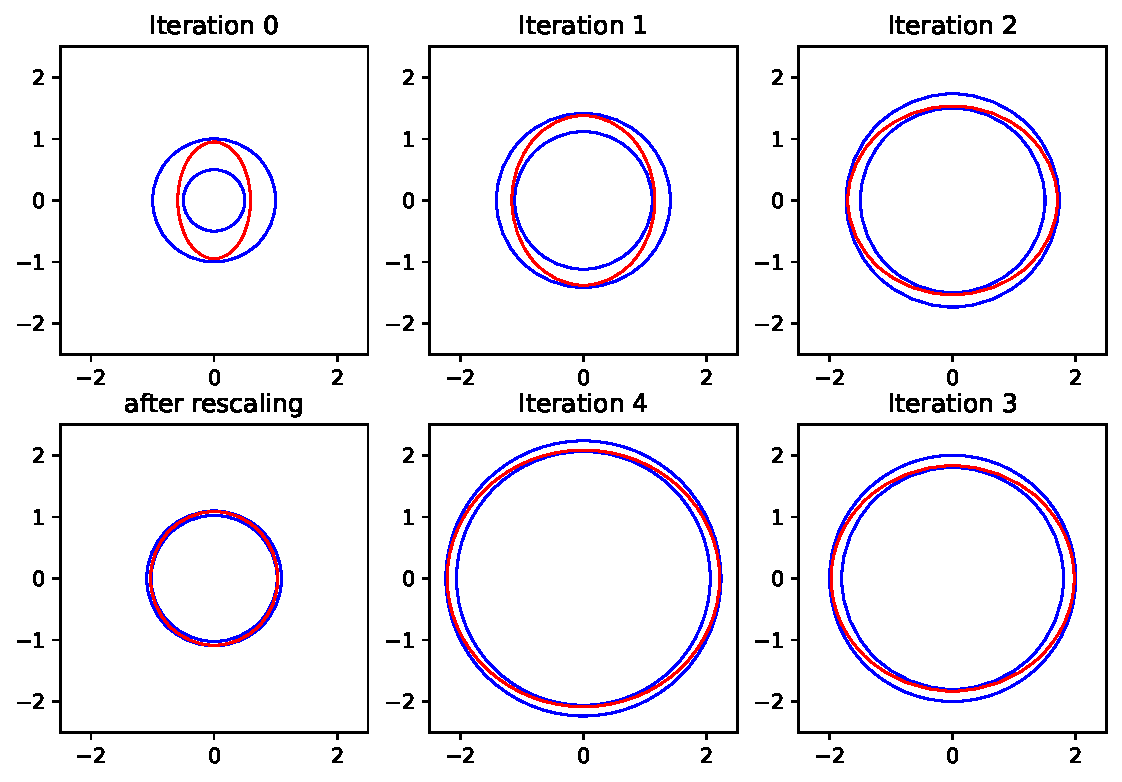
\includegraphics{index_files/figure-pdf/fig-ellipsoid-output-1.pdf}

}

\caption{\label{fig-ellipsoid}The geometric intuition behind the
algorithm.}

\end{figure}

\hypertarget{physical-view-and-the-expected-behavior}{%
\subsection{Physical View and the Expected
behavior}\label{physical-view-and-the-expected-behavior}}

The fact that \(X^{(i)}\) should be bounded between two spheres
translates into all the eigenvalues of \(X^{(i)}\) being bounded between
the two radiuses except for the trivial eigenvalues that their
corresponding eigenvector is in the null-space of \(\Pi\). For
Laplacians, this corresponds to the all one's vector which is in the
null-space of \(L_G\) and \(\Pi = L_G^{+/2} L_G L_G^{+/2}\). For
simplicity, we assume that all the matrices are full rank and
\(\Pi = I\). Using this, we can establish theories that easily
generalize to the case where \(\Pi\) is not the identity matrix via
projection.

An important observation is to monitor what happens to the eigenvalues
of \(X^{(i)}\) when \(vv^T\) is being added at each iteration. To do so,
we consider the characteristic polynomial of \(X\) at each iteration
written as \(p_X(\lambda) = \det(\lambda I - X)\). There are two
important lemmas when analyzing \(A + vv^T\) matrices, one is the
Sherman-Morrison lemma which states that:

\leavevmode\vadjust pre{\hypertarget{lem-sherman-morrison}{}}%
\begin{lemma}[]\label{lem-sherman-morrison}

Suppose \(A\) is an invertible square matrix and \(u, v\) are column
vectors. Then \(A + uv^T\) is invertible iff
\(1 + v^T A^{-1} u \neq 0\). In this case,
\[(A + uv^T)^{-1} = A^{-1} - \frac{A^{-1}uv^TA^{-1}}{1 + v^TA^{-1}u}\]

\end{lemma}

The other is the matrix determinant lemma which states that:

\leavevmode\vadjust pre{\hypertarget{lem-matrix-determinant}{}}%
\begin{lemma}[]\label{lem-matrix-determinant}

Suppose \(A\) is an invertible square matrix and \(u, v\) are column
vectors. Then \[\det(A + uv^T) = \det(A) (1 + v^T A^{-1} u)\]

\end{lemma}

Moreover, plugging these into the characteristic polynomial of
\(X + vv^T\) yields the following:

\begin{align*}
p_{X + vv^T}(\lambda) &= \det(\lambda I - X - vv^T) \\
& = \det(\lambda I - X) (1 - v^T \left(\lambda I - X \right)^{-1}u) \\
& = \det (\lambda I - X) \left(1 - v^T \left[\sum_{i=1}^n \frac{1}{\lambda - \lambda_i} u_i u_i^T\right] v\right)\\
& = p_X(\lambda) \left(1 -  \sum_{i=1}^n \frac{(v^Tu_i)^2}{\lambda - \lambda_i}\right)\\
\end{align*}

Furthermore, we can assume particles being set on certain points of the
\(x\)-axis with the \(i\)th one on \(\lambda_i\) having a charge equal
to \((v^Tu_i)^2\). The new set of equilibrium points for this particle
set will entail the new eigenvalues of \(X + vv^T\) which are the roots
of \(p_{X + vv^T}(\lambda)\). Note that for \(u_i\) values such that
\(v^Tu_i=0\) the charge is zero and therefore, the new eigenvalues will
be the same as the old ones.

The following figure illustrates the matrix case \(X\) with three
different vectors \(v_1\), \(v_2\) and \(v_3\). Each color corresponds
to the characteristic polynomial for different \(v\) values where,

\[X = \lambda_1 u_1 u_1^T + \lambda_2 u_2 u_2^T + \lambda_3 u_3 u_3^T
 = \begin{bmatrix}
1.6 & -0.2 & -0.33\\
-0.2 & 3.4 & -0.33\\
-0.33 & -0.33 & 1
\end{bmatrix}\]
\[\begin{bmatrix}\lambda_1 \\ \lambda_2 \\ \lambda_3\end{bmatrix} = \begin{bmatrix}0.79 \\ 1.75 \\ 3.46\end{bmatrix}, u_1 = \begin{bmatrix}
-0.41\\
-0.15\\
-0.9
\end{bmatrix}, u_2 = \begin{bmatrix}
-0.9 \\
-0.03 \\
0.42
\end{bmatrix}, u_3 = \begin{bmatrix}
0.08\\
-0.99\\
0.12\\
\end{bmatrix}\] We note that \(\langle v_i, u_j \rangle^2\) is the
charge of particle \(j\) when adding \(v_i\) to \(X\) and we can
summarize all the charged particles in the following matrix:
\[v_1 = \begin{bmatrix}
0\\
1\\
1\\
\end{bmatrix}, v_2 = \begin{bmatrix}
1\\
1\\
0\\
\end{bmatrix}, 
C = \begin{bmatrix}
1.10 & 0.15 & 0.75\\
0.31 & 0.87 & 0.82
\end{bmatrix}, C_{ij} = \langle v_i, u_j \rangle^2\]

\begin{figure}

\begin{minipage}[t]{0.50\linewidth}

{\centering 

\raisebox{-\height}{

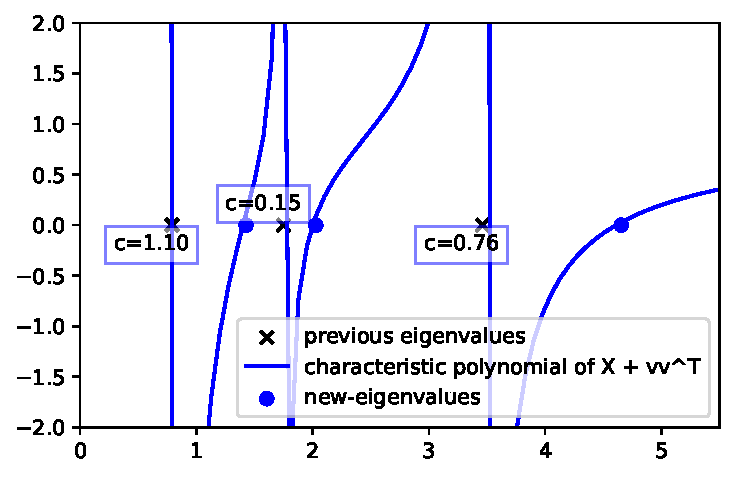
\includegraphics{index_files/figure-pdf/fig-matrix-determinant-output-1.pdf}

}

}

\subcaption{\label{fig-matrix-determinant-1}The characteristic
polynomial after adding \(v_1\) to X.}
\end{minipage}%
%
\begin{minipage}[t]{0.50\linewidth}

{\centering 

\raisebox{-\height}{

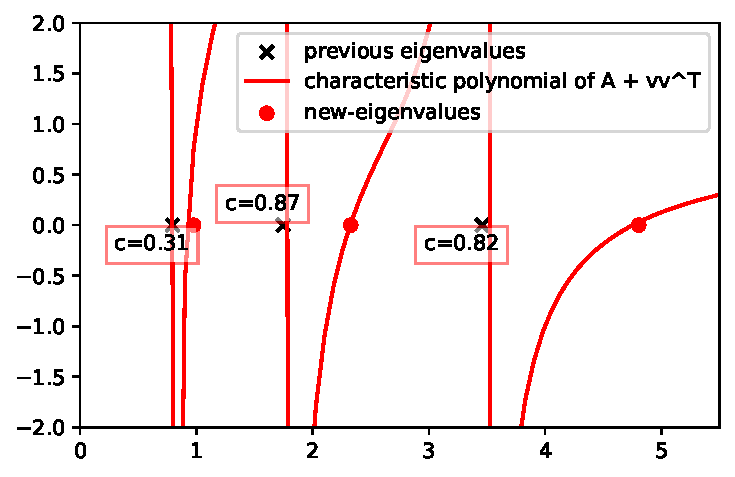
\includegraphics{index_files/figure-pdf/fig-matrix-determinant-output-2.pdf}

}

}

\subcaption{\label{fig-matrix-determinant-2}The characteristic
polynomial after adding \(v_2\) to X.}
\end{minipage}%

\caption{\label{fig-matrix-determinant}The characteristic polynomial of
\(X + vv^T\) for different \(v\) values, the higher the charge the more
it will repel the new eigenvalues from the old ones.}

\end{figure}

The goal is to pick a \(v\) such that the particles are set in a way
that all the eigenvalues are uniformly pushed forward so that they can
stay between the new ranges \(l^{(i+1)}\) and \(u^{(i+1)}\). To get a
sense, let's pick one of the \(m\) vectors with uniform probability and
add it to \(X\). In that case, the expected charges can be written as:
\[E[\langle v, u_j \rangle^2] = \frac{1}{m} \sum_{i=1}^m \langle v_i, u_j \rangle^2 = \frac{1}{m} u_j^T \left( \sum_{i=1}^m v_i v_i^T \right)u_j = \frac{||\Pi u_j||_2^2}{m} = \frac{1}{m}\]
Hence, on expectation, all the particles have a charge of \(1/m\) and
the expected deterministic polynomial is:

\begin{align*}
E[p_{X + v}(\lambda)] &= p_X(\lambda) E\left[1 - \sum_{i=1}^m \frac{\langle u_i, v\rangle^2}{\lambda - \lambda_i}\right] = p_X(\lambda) \left(1 - \sum_{i=1}^m \frac{E\langle u_i, v\rangle^2}{\lambda - \lambda_i}\right)\\
& = p_X(\lambda) \left(1 - \sum_{i=1}^m \frac{1/m}{\lambda - \lambda_i}\right) = p_X(\lambda) - \frac{1}{m} \sum_{i=1}^m \frac{p_X(\lambda)}{\lambda - \lambda_i}\\
& = p_X(\lambda) - \frac{1}{m} \sum_{i=1}^m \prod_{1 = j\neq i}^m (\lambda - \lambda_j)\\
&= p_X(\lambda) - \frac{1}{m} p'_X(\lambda)\\
\end{align*}

Therefore, if we start with the matrix
\(p_{X^{(0)}}(\lambda) = \lambda^n\), after \(nd\) iterations the
expected polynomial is a set of associate Laguerre polynomials that are
well studied (Dette and Studden 1995), and in particular, it has been
proven that the ratio between the largest and smallest root for these
polynomials is bounded by the value below:

\[\frac{d + 1 + 2\sqrt{d}}{d + 1 - 2\sqrt{d}} \xrightarrow{\epsilon = \frac{2\sqrt{d}}{d+1}} \frac{1 + \epsilon
}{1 - \epsilon}\]

Although this is just speculation and no \(v_i\) values will necessarily
exist with the expected behavior, we can still get an idea of the goal
\(\epsilon\) and come up with the following proposition:

\leavevmode\vadjust pre{\hypertarget{prp-final-form}{}}%
\begin{proposition}[]\label{prp-final-form}

For any matrix \(A = \sum_{i=1}^m v_i v_i^T\) we can choose a subset
\(\mathcal{S}\) of \(v_i\) and a set of coefficients \(s_i\) with size
\(nd\) such that:
\[\hat{A} = \sum_{i \in \mathcal{S}} s_i \cdot v_i v_i^T,~~ (1 - \frac{2\sqrt{d}}{d+1}) A \preceq \hat{A} \preceq (1 + \frac{2\sqrt{d}}{d+1}) A\]

\end{proposition}

The graph formulation of Proposition~\ref{prp-final-form} is as follows:

\leavevmode\vadjust pre{\hypertarget{cor-final-form}{}}%
\begin{corollary}[]\label{cor-final-form}

For any graph \(G\) and any \(\epsilon\) we can choose a subset of
\(\mathcal{O}(n/\epsilon^2)\) edges with arbitrary edge weights to
obtain \(H\) such that \(H\) is an \(\epsilon\)-sparsifier of \(G\):
\(L_G \approx_\epsilon L_H\).

\end{corollary}

This is set using \(\epsilon = \frac{2\sqrt{d}}{d + 1}\) where
\(\frac{n}{\epsilon^2} = \mathcal{O}(nd)\). In the next section, we will
see how we can choose \(v_i\) and \(s_i\) at each step such that after
\(nd\) iterations this happens.

\hypertarget{potential-functions}{%
\subsubsection{Potential Functions}\label{potential-functions}}

The big question is, how can we quantize the boundedness of the matrix
\(X\) at each step? We want \(X^{(i)}\) to have eigenvalues that are
bounded by \(l^{(i+1)}\) and \(u^{(i+1)}\); and so, we use a family of
\textbf{potential functions} that explode when the eigenvalues approach
the bounds. A set of such potentials can be chosen using the fact that
\(uI - X\) or \(A - lX\) will have infinitely small eigenvalues when the
eigenvalues of \(X\) approach \(u\) or \(l\) respectively; therefore,
their inverse will be ill-conditioned and have infinitely large
eigenvalues. We can use the following potential functions:

\[\Phi^u_l(X) = \Phi^u(X) + \Phi_l(X) = Tr[(uI - X)^{-1}] + Tr[(X - l I)^{-1}]\]

In summary, the main idea is to choose \(v_i\) and \(s_i\) such that the
potential for the matrix \(X^{(i)}\) in the next iteration does not
explode. To do so, we can ensure that the potentials remain
monotonically decreasing:

\[\infty \gg \Phi^{u^{(0)}}(X^{(0)}) \ge \Phi^{u^{(1)}}(X^{(1)}) \ge ... \ge \Phi^{u^{(nd)}}(X^{(nd)})\]
\[\infty \gg \Phi_{\ell^{(0)}}(X^{(0)}) \ge \Phi_{\ell^{(1)}}(X^{(1)}) \ge ... \ge \Phi_{\ell^{(nd)}}(X^{(nd)})\]

With that in mind, let's assume we are going to assign \(s_k\) to any
vector \(v_k\) such that after the increase in our upper and lower
bound, the potential remains non-increasing. Now let us separately
consider the upper and lower bound potentials.

When increasing \(l^{(i)}\), the eigenvalues come closer to the lower
bound, and hence, the potential of the lower bound will increase;
therefore, for any vector \(v_k\), the coefficient \(s_k\) should be
bounded by some value \(L_{X^{(i)}}(v_k)\) such that after adding
\(s_k \cdot v_k v_k^T\) to \(X^{(i)}\), spectrum shifts forward and the
increase in the potential cancels out. That said, for any matrix \(X\)
and any vector \(v\) we have:

\begin{align*}
&\Phi^{\overset{l'}{\overbrace{l + \delta_l}}}(X + s \cdot vv^T) \le \Phi^l(X)\\
\Phi_{l'}(X + s \cdot vv^T) & = Tr(X + s \cdot vv^T - l'I)^{-1}  \qquad \text{Sherman-Morrison}\\
& = Tr\left((X - l'I)^{-1}\right) + Tr\left(\frac{s \cdot (X - l'I)^{-1} v v^T (X - l'I)^{-1}}{1 + s \cdot v^T (X - l' I)^{-1} v}\right)\\
&= \Phi_{l'}(X) - \frac{s \cdot v^T (X - l'I)^{-2}v}{1 + s \cdot v^T  (X - l'I)^{-1}v} \le \Phi^l(X)
\end{align*}

\begin{align*}
\Leftrightarrow &~ \underset{\Delta}{\underbrace{\Phi_{l'}(X) - \Phi^l(X)}} \le \frac{s \cdot v^T (X - l'I)^{-2}v}{1 + s \cdot v^T  (X - l'I)^{-1}v}\\
\Leftrightarrow &~ s\cdot \left[v^T (X - l'I)^{-2}v  - \Delta v^T(X - l' I)^{-1} v\right] \ge \Delta \\ 
\Leftrightarrow &~ s \ge \frac{\Delta}{v^T \left( (X - l'I)^{-2} - \Delta (X - l' I)^{-1} \right) v} = L_X(v)
\end{align*}

which means,

\begin{equation} \tag{1}\label{eq:lower-bound-potential}
s \ge L_X(v) = \frac{\Delta}{v^T \left((X - l' I)^{-2} - \Delta (X - l' I)^{-1} \right) v}
\end{equation}

On the other hand, a similar thing can be said for the upper-bound
potential. when increasing \(u^{(i)}\), the eigenvalues are further away
from the upper bound which gives us the freedom to shift the eigenvalues
forward. However, this shifting should not be so extreme that the
potential at most increases to offset the decrease introduced after
adding \(\delta_u\) to \(u^{(i)}\): \[ 
\Phi^{\overset{u'}{\overbrace{u + \delta_u}}}(A + s \cdot vv^T) \le \Phi^u(A).
\] Similar to \(\eqref{eq:lower-bound-potential}\), if we negate \(s\)
and \(A\) then the upper-bound potential will act similarly to the
lower-bound potential. Therefore, we can write the following:

\begin{equation} \tag{2}\label{eq:upper-bound-potential}
s \le U_X(v) = \frac{\Delta}{v^T \left((u' I - X)^{-2} - \Delta (u' I - X)^{-1}\right)v}
\end{equation}

Where \(\Delta\) is the difference between \(\Phi^u(X)\) and
\(\Phi^{u'}(X)\).

Finally, for every vector \(v_i\) at each step, we can introduce an
upper and lower bound for the coefficient corresponding to that vector.
However, this is not enough to ensure that at least one \(v_i\) exists
such that \(L_X(v_i) \le U_X(v_i)\); in other words, it might be the
case that for each vector the upper and lower bounds are contradictory
which will put the algorithm in a stale-mate state. To avoid this, we
pick the values \(\delta_u\) and \(\delta_l\) carefully and introduce a
nice lemma in the next section that ensures such a vector always exists.

\hypertarget{the-existence-of-a-good-vector}{%
\subsubsection{The Existence of a good
Vector}\label{the-existence-of-a-good-vector}}

We will now present the following lemma, that for the potentials having
a certain condition, a good vector \(v_k\) and a good coefficient
\(s_k\) always exist. This is the meat and bones of the algorithm:

\leavevmode\vadjust pre{\hypertarget{lem-good-vector-existance}{}}%
\begin{lemma}[]\label{lem-good-vector-existance}

For any set of vectors \(\langle v_1, v_2, ..., v_m \rangle\) that sum
up to an idempotent matrix \(\Pi = \sum v_i v_i^T\) and a matrix \(X\)
being an arbitrary linear combination of their rank one cross product,
if \(\Phi^u(X) \le \epsilon_U\) and \(\Phi_l(X) \le \epsilon_L\) and
\(\epsilon_u, \epsilon_l, \delta_u, \delta_l\) satisfy the following
conditions:
\[0 \le \delta_u^{-1} + \epsilon_u \le \delta_l^{-1} - \epsilon_l,\]
Then, there exists a vector \(v_k\) such that: \[L_X(v_k) \le U_X(v_k)\]
, and hence, by adding \(s \cdot v_k v_k^T\) to \(X\) for
\(s \in [L_A(v_k), U_A(v_k)]\), we can ensure that
\(\Phi^{u + \delta_u}(X + s \cdot v_k v_k^T) \le \Phi^{u}(X)\) and
\(\Phi_{l + \delta_l}(X + s \cdot v_k v_k^T) \le \Phi_l(X)\).

\end{lemma}

\begin{solution}

The proof idea is to show that the sum of all the lower bound values for
all the vectors \(v_k\) is less than or equal to the sum of all the
upper bounds for all vectors \(v_k\). In other words,
\[\sum_{k=1}^m L_X(v_k) \le \sum_{k=1}^m U_X(v_k)\] The proof in
(Batson, Spielman, and Srivastava 2009) shows that the left-hand-side is
bounded by \(\frac{1}{\delta_l^{-1} - \epsilon_l}\) and the
right-hand-side is bounded by \(\frac{1}{\delta_u^{-1} + \epsilon_u}\).
Therefore, the lemma is proven using the conditions mentioned.

To show these two bounds, a lot of algebra is required. The proof is
hidden here for brevity but you can check out the proof of Lemma 3.5 and
Claim 3.6 in (Batson, Spielman, and Srivastava 2009) for more details;
although, they have used a different notation and instead of bounding
\(s_k\) values they bound their reciprocals.

\end{solution}

Now we should pick values that adhere to the conditions:
\[\delta_l = 1, \delta_u = \frac{\sqrt{d} + 1}{ \sqrt{d} - 1}, l^{(0)} = -n \sqrt{d}, u^{(0)} = \frac{n(d+\sqrt{d})}{(\sqrt{d} -1)}\]

Note that in this case, in the first step (starting off with
\(X^{(0)} = 0\)), the upper and lower potentials are upper-bounded as
follows:
\[\Phi^u(X^{(0)}) = Tr(u^{(0)}I)^{-1} = \frac{n}{u^{0}} = \frac{\sqrt{d} - 1}{\sqrt{d} + d} = \epsilon_u\]
\[\Phi_l(X^{(0)}) = Tr(-l^{(0)} I)^{-1} = \frac{n}{l^{0}} = \frac{1}{\sqrt{d}} = \epsilon_l\]

Hence, if we plug in the criteria we have, \[
0 \le 
\frac{d-1}{d + \sqrt{d}} = \underset{\delta_u^{-1}}{\underbrace{\frac{\sqrt{d} - 1}{\sqrt{d} + 1}}} + \underset{\epsilon_u}{\underbrace{\frac{\sqrt{d}-1}{\sqrt{d}+d}}} = \underset{\delta_l^{-1}}{\underbrace{1}} - \underset{\epsilon_l}{\underbrace{\frac{1}{\sqrt{d}}}} = \frac{\sqrt{d} - 1}{\sqrt{d}}
\] which is satisfactory.

Finally, we know that after \(nd\) iterations \(X^{(nd)}\) will be
bounded between the two following spheres:

\begin{align*}
&~~(l^{(0)} + nd \cdot \delta_l) I \preceq X^{(nd)} \preceq (u^{(0)} + nd \cdot \delta_u) I\\
\Leftrightarrow & ~~ (nd - n \sqrt{d}) I \preceq X^{(nd)} \preceq \left(\frac{nd (\sqrt{d} + 1)}{\sqrt{d} - 1} + \frac{n(d + \sqrt{d})}{\sqrt{d} - 1}\right) I
\end{align*}

Then by rescaling both sides of the equations by
\(\gamma = \frac{\sqrt{d} - 1}{n(d+1)\sqrt{d}}\), we have that,

\begin{equation} \tag{3} \label{eq:rescaling}
(1 - \frac{2\sqrt{d}}{d+1}) I \preceq \gamma \cdot X^{(nd)} \preceq (1 + \frac{2\sqrt{d}}{d+1}) I
\end{equation} If we multiply both sides with \(A^{+/2}\) and setting
\(\epsilon = \frac{2\sqrt{d}}{d + 1}\), we get that, \[
(1 - \epsilon) A \preceq \gamma \cdot A^{1/2} X^{(nd)} A^{1/2} \preceq (1 + \epsilon) A
\] In turn, \(A^{1/2} X^{(nd)} A^{1/2}\) would give us the Laplacian
\(L_H\) in the original problem.

\hypertarget{the-deterministic-algorithm}{%
\subsubsection{The Deterministic
Algorithm}\label{the-deterministic-algorithm}}

Now that we have a general sense of the algorithm, we can do a recap of
what the algorithm does:

\begin{enumerate}
\def\labelenumi{\arabic{enumi}.}
\item
  We will first map each edge to a vector
  \(v_e = \sqrt{w_e} L_G^{+/2} (\chi_{e_1} - \chi_{e_2})\) where \(w_e\)
  is the weight of the edge and \(\chi_{e_i}\) is the indicator vector
  of the vertex \(e_i\).
\item
  We start with the all-zeros matrix \(X\) which is intended to
  approximate the spherically shaped idempotent matrix
  \(\Pi = L_G^{+/2} L_G L_G^{+/2}\).
\item
  To do so, we run \(nd\) iterations and pick an edge corresponding to a
  vector \(v_i\) in each iteration such that the potentials remain
  monotonically non-increasing.

  \begin{enumerate}
  \def\labelenumii{\roman{enumii}.}
  \tightlist
  \item
    For that, we compute the lower and upper bounds for the
    coefficients. For all the potential computations, we consider the
    edges in the \(n-1\)-dimensional subspace after applying
    \(L_G^{+/2}\) to both sides.
  \item
    We pick a vector \(v_i\) such that the lower bound for that vector
    is less than the upper bound and pick a coefficient between those
    two bounds.
  \end{enumerate}
\item
  We add \(X\) with \(s \cdot v_i v_i\) each step to get a large
  spherical matrix \(X^{(nd)}\).
\item
  Finally we multiply \(L_G^{1/2}\) to both sides of \(X^{(nd)}\) and do
  a rescale to obtain the Laplacian \(L_H\).
\end{enumerate}

\textbf{Complexity Analysis} For analyzing the time complexity, we note
that the reduction takes \(\mathcal{O}(n^3)\) times to compute
\(L^{+/2}\) and \(\mathcal{O}(m \cdot n^2)\) to compute
\(v_i = \sqrt{w_i} L_G^{+/2} L_i\). Then, the algorithm takes
\(\mathcal{O}(nd)\) time to run the iterations and at each iteration
upper bound and lower bound values should be computed for all vectors
\(v_i\). To compute these upper and lower bounds, recall that in both
\(\eqref{eq:upper-bound-potential}\) and
\(\eqref{eq:lower-bound-potential}\) we need to compute the inverse of
\(uI - X^{(i)}\) and \(X^{(i)} - l I\). As a precompute step, we
calculate both of them using \(\mathcal{O}(n^3)\) algorithm and then
compute every upper and lower bound by \(m \times \mathcal{O}(n^2)\)
operations for finding the quadratic form. Therefore, the total time
complexity of the algorithm is
\(\mathcal{O}(n^3 + m \cdot n^2 + nd \cdot m \cdot n^2) = \mathcal{O}(m n^3 d)\).
Although the algorithm is not fast in particular, it is the first
approach that gives near-linear edge counts. Other follow-up works have
produced faster results with (Tat Lee and Sun 2015) giving an almost
linear algorithm to find almost linear sparsifiers.

\hypertarget{experimental-details}{%
\subsubsection{Experimental Details}\label{experimental-details}}

We implemented the algorithm in Python and tested it on a set of graphs.
Our package is available
\href{https://github.com/HamidrezaKmK/twice-ramanujan-sparsifiers}{here}
and Figures~\ref{fig-barbell} and \ref{fig-dumbell} demonstrates the results of the algorithm
on a barbell graph.


\begin{figure}[H]

{\centering 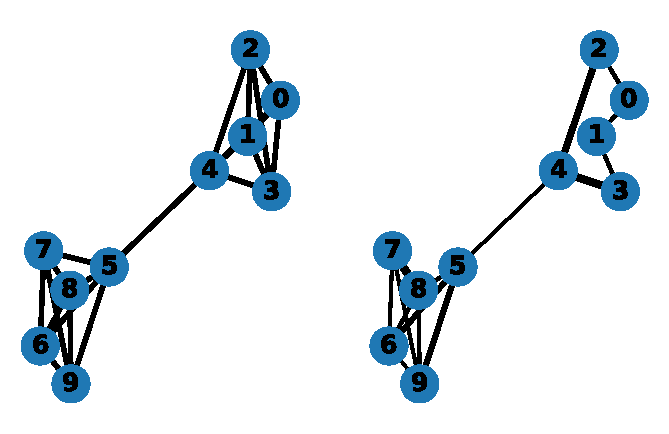
\includegraphics{index_files/figure-pdf/fig-barbell-output-1.pdf}

}

\caption{Checking the algorithm on a barbell graph.}

\label{fig-barbell}
\end{figure}


\begin{figure}[H]

{\centering 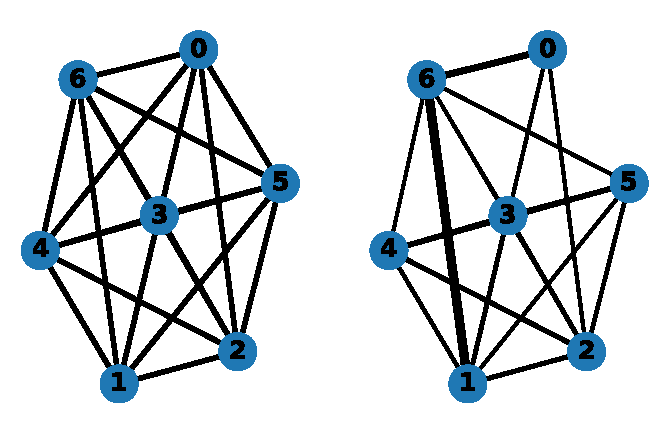
\includegraphics{index_files/figure-pdf/fig-barbell-output-3.pdf}

}
\caption{Checking the algorithm on a complete graph.}

\label{fig-dumbell}
\end{figure}

There were some subtleties in the implementation when numerical issues
were encountered. For example, in the algorithm, we need to compute the
inverse of \(uI - X^{(i)}\) and \(X^{(i)} - l I\) for the upper and
lower bound values. This introduced a lot of accuracy issues, to
circumvent this, we also implemented a binary search-based
implementation to find the upper and lower bound for each vector
\(v_i\); this turned out to be far superior although it impeded the
runtime. You can simply trigger this mode by setting \texttt{fast=True}
in the constructor of \texttt{TwiceRamanujan} class.

\hypertarget{sparsification-of-complete-graphs}{%
\subsection{Sparsification of Complete
Graphs}\label{sparsification-of-complete-graphs}}

Now that we have illustrated the algorithm in its entirety, we will
consider the case of running this sparsifier on the complete graph,
after all, the whole reason behind this naming is its resemblance to the
Ramanujan expanders. But first, let's recap expanders and some of their
properties and then we will see how the sparsifier shares a lot of these
properties.

\hypertarget{expander-graphs}{%
\subsubsection{Expander Graphs}\label{expander-graphs}}

In literature, expander graphs are regular graphs that have high
connectivity; in other words, any random walk on such a graph expands
fast. In many applications like connected computing elements or
communication networks, such highly connected components are required,
but it is always desirable that high connectivity is achieved with
sparse constructions. For example, the complete graphs are an extreme
case of highly connected graphs but are not sparse. Strictly defined,
the expanders are the family of graphs that keep on expanding with high
connectivity but with a sparse number of edges.

Different definitions of expanders are defined using metrics such as
vertex expansion, edge expansion and spectral expansion; we will only
consider the case of spectral expansion here. A definition of
\((d, \epsilon)\)-spectral expanders with a tight connection to the
sparsifiers is given below:

\leavevmode\vadjust pre{\hypertarget{def-spectral-expander}{}}%
\begin{definition}[]\label{def-spectral-expander}

A \(d\)-regular graph \(G\) is a \((d, \epsilon)\)-spectral expander if
it approximate the complete graph \(K_n\) in a spectral sense, in other
words,
\[(1 - \epsilon) L_{K_n} \preceq \frac{n}{d} L_G \preceq (1 + \epsilon) L_{K_n}\]

\end{definition}

\hypertarget{expander-mixing-properties}{%
\paragraph{Expander Mixing
Properties}\label{expander-mixing-properties}}

A well-known theorem in the literature is the expander mixing lemma,
which states that the edges of a spectral expander are distributed
uniformly across the graph. This is a very important property of the
expanders, as it allows us to use the sparsifiers to approximate the
complete graph. The expander mixing lemma is given below:

\leavevmode\vadjust pre{\hypertarget{thm-expander-mixing-lemma}{}}%
\begin{theorem}[]\label{thm-expander-mixing-lemma}

\textbf{(Expander Mixing Lemma)} Let \(G\) be a
\((d, \epsilon)\)-spectral expander. Then for any two disjoint sets
\(S\) and \(T\) of vertices, we have,
\[|E_G(S, T) - \frac{d}{n} |S| \cdot |T| | \le \epsilon \sqrt{|S| \cdot |T|}\]

\end{theorem}

This means that if we multiply the edges of an expander by \(n/d\) so
that it becomes a sparsifier of the complete graph and call it \(H\),
then the following holds:
\[|E_H(S, T) - |S| \cdot |T|| \le \epsilon \frac{n}{d} \cdot \sqrt{|S| \cdot |T|}\]

That said, even though twice Ramanujan sparsifiers are not expanders
(they are not regular) we have the following lemma for spectral
sparsifiers that bear resemblance to the expander mixing lemma:

\leavevmode\vadjust pre{\hypertarget{thm-approx-mixing-lemma}{}}%
\begin{theorem}[]\label{thm-approx-mixing-lemma}

Let \(L_H(V,E,w)\) be a graph that \((1+\epsilon)\) approximates the
complete graph \(L_G\) then for every pair of disjoint sets S and T, \[
|E(S,T)-(1+\epsilon/2)|S||T||\leq n(\epsilon/2) \sqrt{|d||n|}
\]

\end{theorem}

\begin{solution}

Through the definition we have \[
  -\frac{\epsilon}{2} L_G \preceq L_H-(1+\epsilon/2)L_G \preceq \frac{\epsilon}{2} L_G
\]

So it is possible to write it as \[
  L_H=(1+\epsilon/2)L_G+X_M
\] where \(X_M\) is calculated based on norms with it having max norm as
\(\frac{\epsilon}{2} ||L_G|| \leq n\epsilon/2\) Now consider \(x\) and
\(y\) as characteristic vectors of set \(S\) and \(T\) respectively. As
we know \(-E(S,T) = x^TL_Hy\) we will get the weight crossing the two
sets. And we consider with a complete graph, the weight is uniformly
distributed \[x^TL_Gy= -|S||T|\] Substituting back
\[x^TL_Hy = (1+\frac{\epsilon}{2}x^TL_Gy+x^TX_my)\]
\[x^TL_Hy = (1+\frac{\epsilon}{2}|S||T|+x^TX_my)\]
\[-(E(S,T) -(1+\frac{\epsilon}{2}|S||T|)= x^TX_my)\] Taking modulus on
both sides \[|E(S,T) -(1+\frac{\epsilon}{2})|S||T||= |x^TX_my|\]
Consider RHS and apply the Cauchy-Schwarz inequality
\[|x^TX_my|\leq||X_m||\:||x||\:||y||\leq n\frac{\epsilon}{2}\sqrt{|S||T|}\]
Substituting back
\[|E(S,T) -(1+\frac{\epsilon}{2})| \leq n\frac{\epsilon}{2}\sqrt{|S||T|}\]

\end{solution}

That said, the twice Ramanujan can be a good approximate for the
complete graph and any vertex set will expand. Now let's move on to
Ramanujan bounds.

\hypertarget{ramanujan-bounds}{%
\subsubsection{Ramanujan Bounds}\label{ramanujan-bounds}}

For expanders, we know that the higher \(d\) the more freedom we have to
choose more dense graphs that give us better approximations resulting in
lower values of \(\epsilon\). That said, given a specific value of
\(d\), there exist some lower bounds on the accuracy metric
\(\epsilon\). Intuitively, the lower the value of \(d\), the worst the
accuracy gets and \(\epsilon\) should increase. The Alan-Bopanna lemma
bridges that gap between these two concepts and states a lower limit for
the second eigenvalue for the Laplacians of \(d\)-regular graphs: \[
    \lambda_i \geq 2\sqrt{d-1} − o_n(1),
\] and a connected \(d\)-regular graph obtaining this bound is called a
Ramanujan graph. Alternatively, the lemma can produce a bound on the
accuracy metric \(\epsilon\) as follows:
\[\frac{1 + \epsilon}{1 - \epsilon} \ge 1 + \frac{4}{\sqrt{d}} + o_n(1/d)\]
Therefore, Ramanujan graphs are the best-known expanders for a given
value of \(d\). Following the theme of drawing connections between
sparsification and expanders, we can also prove a lower bound for the
accuracy metric \(\epsilon\). With this bound, we can get a sense of how
well a sparsification algorithm acts.

\leavevmode\vadjust pre{\hypertarget{thm-ramanujan-sparsifier-bounds}{}}%
\begin{theorem}[]\label{thm-ramanujan-sparsifier-bounds}

If \(H\) is a graph that \(\epsilon\)-approximates the graph \(G\) such
that \(L_H \approx_\epsilon L_G\), then we have,
\[\frac{1 + \epsilon}{1 - \epsilon} \ge 1 + \frac{2}{\sqrt{d}} - \mathcal{O}\left( \frac{\sqrt{d}}{n} \right)\]
if \(H\) contains a vertex of degree \(d\).

\end{theorem}

\begin{solution}

The key aspect of the proof is the fact that if we consider the Rayleigh
coefficient ratio of \(L_H\) for two different vectors, which are
orthogonal to all 1 vector, it can be at max
\(\kappa = \frac{1 + \epsilon}{1 - \epsilon}\) due to sparsifier
definition.

Now for the construction, consider the d-degree vertex, let it be
\(v_0\), and its neighbors are \(v_1 ....v_n\). Now let the weight of
the edge connecting that neighbor to the \(v_0\) be \(w_i\) and the
weight to all the rest of vertices excluding \(v_0\) neighbors be
\(\delta_i\).

So if we define the characteristic vectors

\[ x(v_i)=\begin {cases} 
      1 & v_i\in v_0 \\
      \frac{1}{\sqrt{d}} & v_i\in {v_1,...v_d} \\
      0 & v_i\notin {v_0,v_1...v_d} 
   \end{cases}
\]

\[ y(v_i)=\begin {cases} 
      1 & v_i\in v_0 \\
      -\frac{1}{\sqrt{d}} & v_i\in {v_1,...v_d} \\
      0 & v_i\notin {v_0,v_1...v_d} 
   \end{cases}
\] Now taking quadratic forms concerning these and using the edge
definition of laplacian \[
x^TL_Hx = \sum^{d}_{i=1}w_i(1-1/\sqrt(d))^2+\sum^d_{i=1}\delta_i(1/\sqrt(d)-0)^2 
\] \[
 = \sum^{d}_{i=1}w_i+\sum^{d}_{i=1}\frac{\delta_i+w_i}{d}-2\sum^d_{i=1}\frac{w_i}{\sqrt{d}} 
\]

Similarly for y \[
y^TL_Hy = \sum^{d}_{i=1}w_i+\sum^{d}_{i=1}\frac{\delta_i+w_i}{d}+2\sum^d_{i=1}\frac{w_i}{\sqrt{d}} 
\] Now taking ratio
\[\frac{y^TL_Hy}{x^TL_Hx}=\frac{1+\frac{1}{\sqrt{d}}\frac{2\sum^d_{i=1}w_i}{\sum^{d}_{i=1}w_i+\sum^{d}_{i=1}\frac{\delta_i+w_i}{d}}}{1-\frac{1}{\sqrt{d}}\frac{2\sum^d_{i=1}w_i}{\sum^{d}_{i=1}w_i+\sum^{d}_{i=1}\frac{\delta_i+w_i}{d}}}\]

Now consider the lower bound for L\_H defined earlier. Now consider a
vertex and define a characteristic vector concerning its neighbors,
i.e.~only the position corresponding to these neighbors be 1 and the
rest 0. The quadratic form, which will be the weighted degree of the
graph, will be bounded between n \(n\kappa\). So using this \[
\frac{2\sum^d_{i=1}w_i}{\sum^{d}_{i=1}w_i+\sum^{d}_{i=1}\frac{\delta_i+w_i}{d}}= \frac{2}{1+\frac{\sum^{d}_{i=1}\frac{\delta_i+w_i}{d}}{\sum^d_{i=1}w_i}} \geq \frac{2}{1+\kappa}
\] thus
\[\frac{y^TL_Hy}{x^TL_Hx}\geq \frac{1+\frac{1}{\sqrt{d}}\frac{2}{1+\kappa}}{1-\frac{1}{\sqrt{d}}\frac{2}{1+\kappa}}
\] Since the L\_H's quadratic form bound between the lowest possible
value n and highest possible value \(n\kappa\) is only true for vectors
orthogonal to all single constant vectors. So transforming variables to
such space \[
||x^*|| = ||x||^2-(<x,1/\sqrt{n}>)^2 = 2-\frac{(1-\sqrt{d})^2}{n}
\] \[
||y^*|| = ||y||^2-(<y,1/\sqrt{n}>)^2 = 2-\frac{(1-\sqrt{d})^2}{n}
\]

taking ratio
\[\frac{||x^*||}{||y^*||} = 1- \frac{4\sqrt{d}}{2-\frac{(1-\sqrt{d})^2}{n}}
\] \[
\frac{||x^*||}{||y^*||} = 1- O(\frac{\sqrt{d}}{n})
\] Changing variables for quadratic form ratio

\[\frac{y^TL_Hy}{x^TL_Hx}\frac{||x^*||}{||y^*||}\geq \frac{1+\frac{1}{\sqrt{d}}\frac{2}{1+\kappa}}{1-\frac{1}{\sqrt{d}}\frac{2}{1+\kappa}}(1- O(\frac{\sqrt{d}}{n}))
\] maximum value for LHS due to lower bound is \(\kappa\)
\[\kappa\geq \frac{1+\frac{1}{\sqrt{d}}\frac{2}{1+\kappa}}{1-\frac{1}{\sqrt{d}}\frac{2}{1+\kappa}}(1- O(\frac{\sqrt{d}}{n}))
\]
\[\frac{y^TL_Hy}{x^TL_Hx}\frac{||x^*||}{||y^*||}\geq \frac{1+\frac{1}{\sqrt{d}}\frac{2}{1+\kappa}}{1-\frac{1}{\sqrt{d}}\frac{2}{1+\kappa}}(1- O(\frac{\sqrt{d}}{n}))
\] which finally transforms to \[
\kappa \geq 1+2/\sqrt{d}-O(\sqrt{d}/n)
\]

\end{solution}

That said, the graphs obtained from the twice Ramanujan algorithm
contain \(dn\) edges, which means that using the pigeonhole principle at
least one vertex with a degree at most \(d\) exists. Therefore, any
sparsifier should comply with the bound provided by
Theorem~\ref{thm-ramanujan-sparsifier-bounds}. At the same time, this
bound is somewhat tight as we know that the algorithm produces the
following ratio:
\[\frac{1 + \epsilon}{1 - \epsilon} = \frac{1 + d + 2 \sqrt{d}}{1 + d - 2 \sqrt{d}} =1 + 4\frac{\sqrt{d}}{1 + d - 2\sqrt{d}} \approx 1 + \frac{4}{\sqrt{d}}\]
In addition, Ramanujan graphs in the expander regime have
\(\frac{dn}{2}\) edges while this sparsifier has \(dn\) edges, hence,
the naming convention is set like that.

\hypertarget{conclusions}{%
\subsection{Conclusions}\label{conclusions}}

With that said, we conclude this write-up. Through this, we covered the
following key points:

\begin{enumerate}
\def\labelenumi{\arabic{enumi}.}
\tightlist
\item
  Applications and background of sparsification
\item
  Spectral sparsification
\item
  Reduction from the sparsification problem to the matrix approximation
  problem
\item
  The main method of twice Ramanujan sparsification
\item
  Experimental details and introducing our package
\item
  Drawing connections between sparsified complete graphs and expenders
\item
  measuring how good the sparsifiers are in terms of Ramanujan-like
  bounds.
\end{enumerate}
\newpage
\section{References}
\hypertarget{refs}{}
\begin{CSLReferences}{1}{0}
\leavevmode\vadjust pre{\hypertarget{ref-batson2009twice}{}}%
Batson, Joshua D, Daniel A Spielman, and Nikhil Srivastava. 2009.
{``Twice-Ramanujan Sparsifiers.''} In \emph{Proceedings of the
Forty-First Annual ACM Symposium on Theory of Computing}, 255--62.

\leavevmode\vadjust pre{\hypertarget{ref-benczur1996approximating}{}}%
Benczúr, András A, and David R Karger. 1996. {``Approximating St Minimum
Cuts in {Õ} (n 2) Time.''} In \emph{Proceedings of the Twenty-Eighth
Annual ACM Symposium on Theory of Computing}, 47--55.

\leavevmode\vadjust pre{\hypertarget{ref-cheeger1970lower}{}}%
Cheeger, Jeff. 1970. {``A Lower Bound for the Smallest Eigenvalue of the
Laplacian, Problems in Analysis, a Symposium in Honor of s.''}
\emph{Bochner, Princeton U. Press, Princeton}.

\leavevmode\vadjust pre{\hypertarget{ref-chew1989there}{}}%
Chew, L Paul. 1989. {``There Are Planar Graphs Almost as Good as the
Complete Graph.''} \emph{Journal of Computer and System Sciences} 39
(2): 205--19.

\leavevmode\vadjust pre{\hypertarget{ref-dette1995some}{}}%
Dette, Holger, and William J Studden. 1995. {``Some New Asymptotic
Properties for the Zeros of Jacobi, Laguerre, and Hermite
Polynomials.''} \emph{Constructive Approximation} 11 (2): 227--38.

\leavevmode\vadjust pre{\hypertarget{ref-lee2017sdp}{}}%
Lee, Yin Tat, and He Sun. 2017. {``An Sdp-Based Algorithm for
Linear-Sized Spectral Sparsification.''} In \emph{Proceedings of the
49th Annual Acm Sigact Symposium on Theory of Computing}, 678--87.

\leavevmode\vadjust pre{\hypertarget{ref-li2020sgcn}{}}%
Li, Jiayu, Tianyun Zhang, Hao Tian, Shengmin Jin, Makan Fardad, and Reza
Zafarani. 2020. {``Sgcn: A Graph Sparsifier Based on Graph Convolutional
Networks.''} In \emph{Pacific-Asia Conference on Knowledge Discovery and
Data Mining}, 275--87. Springer.

\leavevmode\vadjust pre{\hypertarget{ref-rudelson1999random}{}}%
Rudelson, Mark. 1999. {``Random Vectors in the Isotropic Position.''}
\emph{Journal of Functional Analysis} 164 (1): 60--72.

\leavevmode\vadjust pre{\hypertarget{ref-spielman2008graph}{}}%
Spielman, Daniel A, and Nikhil Srivastava. 2008. {``Graph Sparsification
by Effective Resistances.''} In \emph{Proceedings of the Fortieth Annual
ACM Symposium on Theory of Computing}, 563--68.

\leavevmode\vadjust pre{\hypertarget{ref-spielman2004nearly}{}}%
Spielman, Daniel A, and Shang-Hua Teng. 2004. {``Nearly-Linear Time
Algorithms for Graph Partitioning, Graph Sparsification, and Solving
Linear Systems.''} In \emph{Proceedings of the Thirty-Sixth Annual ACM
Symposium on Theory of Computing}, 81--90.

\leavevmode\vadjust pre{\hypertarget{ref-spielman2011spectral}{}}%
---------. 2011. {``Spectral Sparsification of Graphs.''} \emph{SIAM
Journal on Computing} 40 (4): 981--1025.

\leavevmode\vadjust pre{\hypertarget{ref-tat2015constructing}{}}%
Tat Lee, Yin, and He Sun. 2015. {``Constructing Linear-Sized Spectral
Sparsification in Almost-Linear Time.''} \emph{arXiv e-Prints},
arXiv--1508.

\end{CSLReferences}



\end{document}
